
\documentclass{report}

\usepackage{alltt,epsf,epsfig,amsmath,amssymb,enumerate,color}
\usepackage{pslatex}
\usepackage{fancybox}

\newcommand{\python}{{\sc Python}}
\newcommand{\logscope}{{\sc LogScope}}
\newcommand{\logscopeSL}{{\sc LogScope/SL}}
\newcommand{\logscopeLog}{{\sc LogScope/LogGenerator}}
\newcommand{\logscopeObserver}{{\sc LogScope/Observer}}
\newcommand{\logscopeLearner}{{\sc LogScope/Learner}}
\newcommand{\ruler}{{\sc Ruler}}
\newcommand{\rmor}{{\sc Rmor}}
\newcommand{\rcat}{{\sc Rcat}}

\newcommand{\todo}[1]{\noindent ----- {\bf #1}}

\newenvironment{code}[1] % uses verbatim
{
\vspace{0.5cm}
\begin{center}
\begin{Sbox}
\begin{minipage}{11cm}
%\begin{verbatim}
\begin{alltt}
{\bf\em #1}
}
{
%\end{verbatim}
\end{alltt}
\end{minipage}
\end{Sbox}
\setlength{\fboxsep}{8pt}
\fbox{\TheSbox}
\end{center}
\vspace{0.5cm}
}

\begin{document}

\begin{figure}
\begin{center}
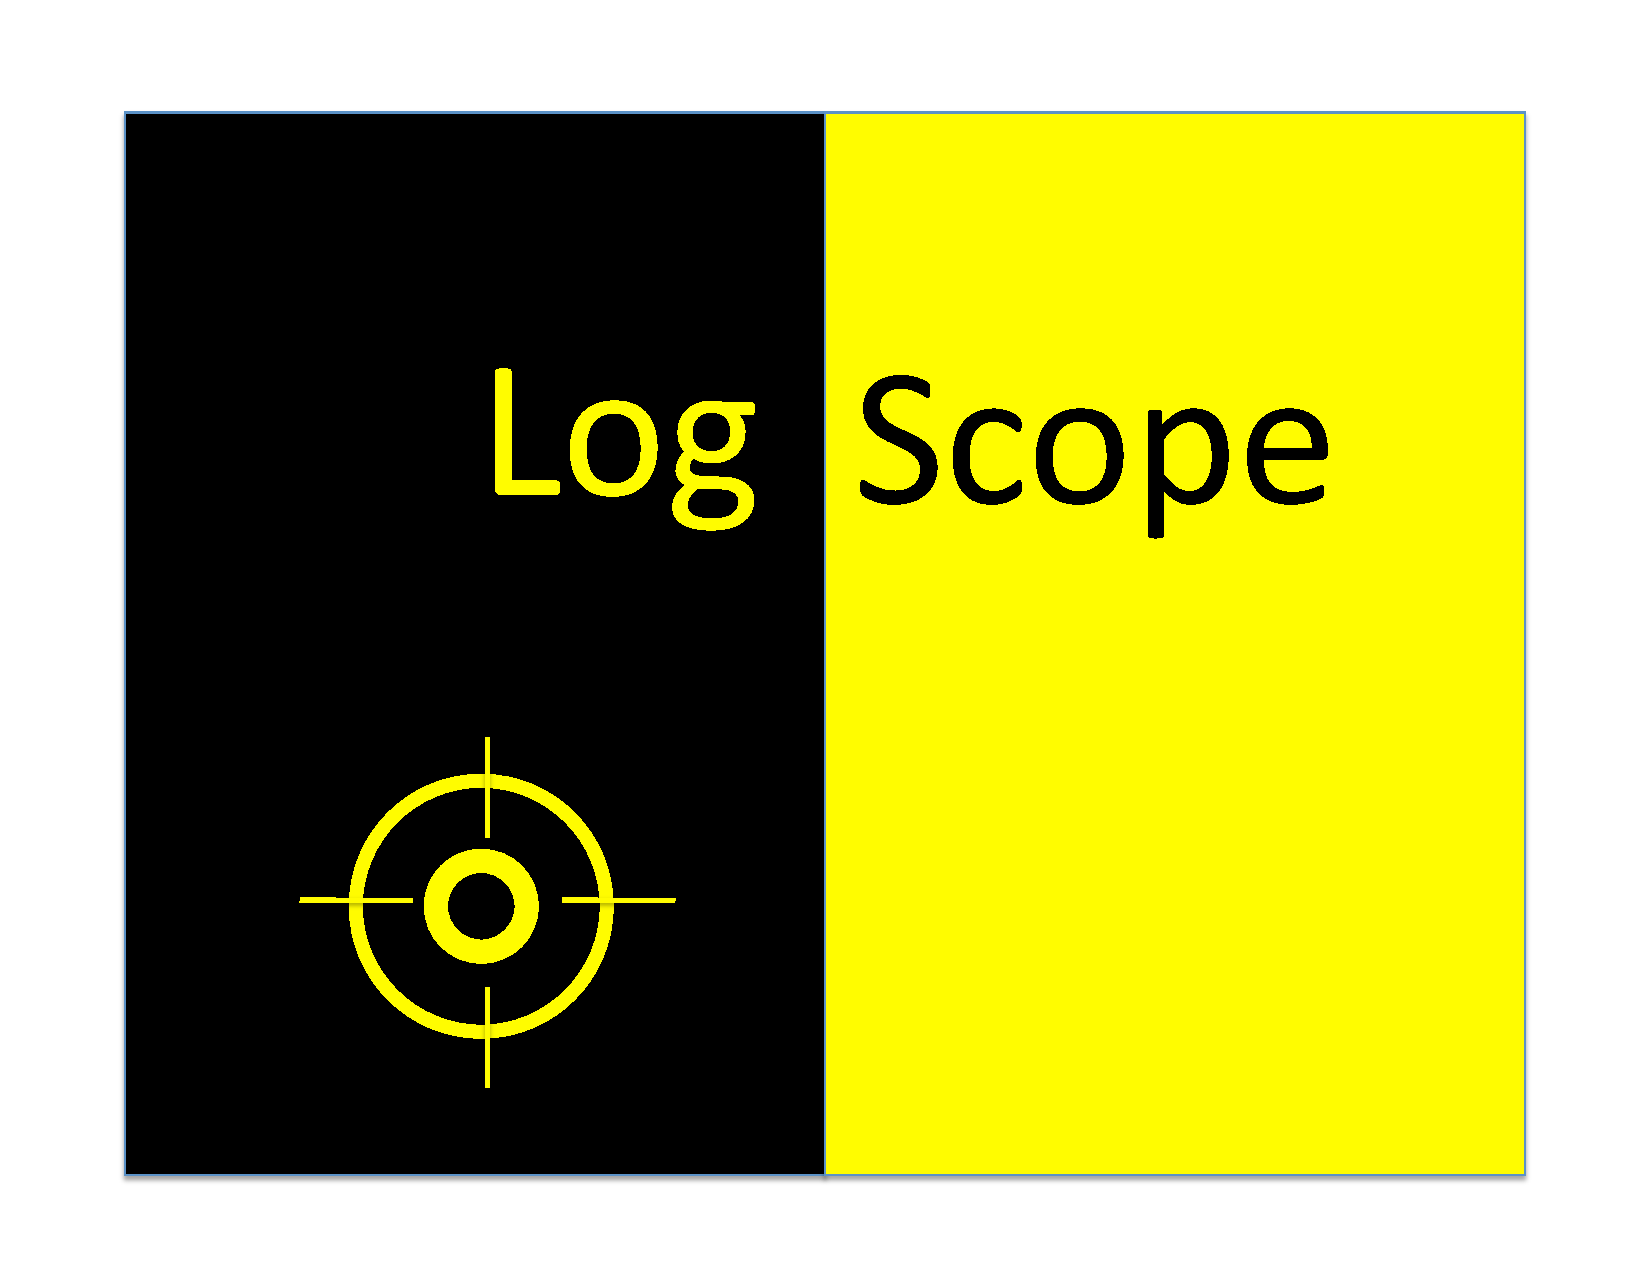
\includegraphics[width=0.5\textwidth]{graphics/logo}
\end{center}
\end{figure}


\title{The \logscope{} Log File Analyzer\\ User Manual}
\author{Klaus Havelund\\ \\
Laboratory for Reliable Software\\
Jet Propulsion Laboratory\\ 
California, USA}

\maketitle


\begin{abstract}

\noindent
This manual explains how to use the \logscope{} log file analysis tool.
\logscope{} has been developed to specifically assist in testing JPL's Mars Science Laboratory (MSL) 
flight software, but is very generic in nature and can in principle be applied to any application that produces 
some form of logging information (which almost any software does). 
The intended use is for offline post-processing of such logs, after execution of the system under test.
\logscope{} processes logs in a specific format (\python{} lists of events). 
The generation of logs in this format from original logcs is beyond the scope of the manual,
but can typically be done with a small \python{} script. 
\logscope{} can in principle also be used to monitor systems online, during their execution. 
However, this will require a different setup of the tool than described in
this manual.  Logs are checked against specifications written in a formalized 
specification language that includes a powerful parameterized extension of state 
machines and a practical and user friendly temporal logic. 
Specifications can furthermore be learned from log files.
The manual explains the specification language and the API.
\end{abstract}

\subsubsection*{Acknowledgements} The following people have had influence on the design of LogScope: Alex Groce (JPL), Margaret Smith (JPL), Howard Barringer (University of Manchester), Chris Delp (JPL), Cin-Young Lee (JPL), and Lisa Tatge (JPL).

\newpage
\tableofcontents

\chapter{Introduction}

\logscope{} is a \python{} program that supports analysis of log files for testing purposes. The tool
in principle takes as input a log file and a specification of expectations wrt. the format of the log file,
and produces as output a report on violations of the specification. A log file is assumed to be a \python{}
sequence containing \python{} dictionaries as events, as explained in this report.
\logscope{} has been developed to specifically assist in testing Mars Science Laboratory (MSL) 
flight software, but is very generic in nature and can in principle be applied to other applications.

The \logscope{} Specification Language (\logscopeSL{}) consists of two parts:
(i) a high-level {\em pattern language}, much resembling a temporal logic, and
(ii) a lower-level, but more expressive, {\em rule language} (we shall often refer to it as the automata language since specifications in this core language resemble familiar automata). 
Patterns are automatically translated to automata. It is the intention that the user should
mostly write patterns, but automata can become necessary in certain cases where the
extra expressive power is needed.
Appendix \ref{app:grammar} contains the full grammar of the total specification language, while
Appendix \ref{app:predicates} contains the list of predefined predicates, which can be used to constrain
events in {\tt where}-clauses.

\subsubsection*{Related Work and Sources of Inspiration}

The \logscope{} system has specifically been influenced by the \ruler{} system
\cite{barringer-ruler-07,barringer-ruler-journal-08,barringer-tutorial-08}, 
and in particular wrt. the rule-based core language. \logscope{} shall really be seen as an adaptation of \ruler{}
to the specific needs of JPL's MSL project by adding temporal logic, making some adjustments, and re-programming in
\python. \logscope{} has, however, also been influenced by
the state machine-based  systems \rcat{} system \cite{smith-havelund-rcat-08} and  \rmor{} \cite{havelund-rmor-08}.
A substantial amount of work has been done on runtime verication within the last decade
\cite{rv}, such as for example \cite{java-mac01}, \cite{statl-01}, \cite{chen-rosu-2007-oopsla}, and \cite{havelund-rosu03c}, all of which has guided in the design of \ruler{} as well as \logscope{}.
 
%Relevant for the temporal pattern language is the set of specifcation patterns collected on
%\cite{patterns05}. 
%Learning is not currently based on the classic work on learning \cite{abgluin-87}, but
%may be.

\chapter{Log Files}
\label{sec:logfiles}

\logscope{} can issue statements about the well-formedness of logs, where a log is a sequence of events.  The kind of log that \logscope{} can process is  more specifically a (\python) sequence of events, where an event is assumed to be a \python{} dictionary: a mapping from field names (strings) to values (strings, integers, floats, even lists). A special field named {\tt "OBJ\_TYPE"} must be defined in all events, and must be mapped to
one of the five string values {\tt "COMMAND"}, {\tt "EVR"}, {\tt "CHANNEL"}, 
{\tt "CHANGE"}, and {\tt "PRODUCT"}, indicating what kind of event it concerns.
These five event kinds correspond to the five kinds of event reports generated by 
MSL\footnote{A soon-to-come version of the tool will be agnostic to the particular kinds of events generated in a log, and hence will not be MSL specific.}, and are explained as follows:

\begin{itemize}
  \item {\tt COMMAND}: commands issued to the spacecraft (input to the system).
  \item {\tt EVR}:  internal transitions, usually generated by logging statements in the code.
  \item {\tt CHANNEL}: periodic samplings of the spacecraft state.
  \item {\tt CHANGE}: delta-changes to the spacecraft state.
  \item {\tt PRODUCT}: science results produced by the software/hardware (output of the system).
\end{itemize}

%In addition to {\tt OBJ\_TYPE}, each event also contains an {\tt EventNumber} field denoting the number of
%the event counted from the first in the log, starting from 1. This information is useful when encountering
%errors for reference. 
\noindent
Although these different event kinds have special meaning for MSL, \logscope{} is agnostic about their meaning.
No other constraints are put on the remaining fields of an event. That is, any event can have any fields from the perspective of \logscope.
%
How log files are generated is beyond the scope of this report. They can for example be
generated from log files or program output generated in some other format, using an
intermediate translating script that converts from the other log file format to the one expected by \logscope{}. Such a script would typically be written in \python{}.

\vspace{0.5cm}

\noindent
The following is an example of a {\em command} event. 

\begin{code}{}
  \{
    "OBJ_TYPE" : "COMMAND",
    "EventNumber" : 12673,
    "String" : "REMS_FP_DMP,0",
    "EventTime" : "2008-295T18:47:52.000",
    "Stem" := "REMS_FP_DMP",
    "SCET" := None,
    "Arguments" := ['0'],
    "Number" := 2,
    "Type" := "FlightSoftwareCommand"
  \}
\end{code}

\noindent We shall as an example consider the following simplified log file consisting of 5 events as basis for a through-going example:

\label{logfile}

\begin{code}{}
  log = 
   [
    \{"OBJ_TYPE" : "COMMAND",  "Type" : "FSW", 
        "Stem" : "PICT", "Number" : 231\},
    \{"OBJ_TYPE" : "EVR",  "Dispatch" : "PICT", "Number" : 231\},
    \{"OBJ_TYPE" : "CHANNEL",  "DataNumber" : 5\},
    \{"OBJ_TYPE" : "EVR",  "Success" : "PICT", "Number" : 231\},
    \{"OBJ_TYPE" : "PRODUCT", "ImageSize" : 1200\}
   ]
\end{code}

\noindent The log could correspond to the command {\tt "PICT"} to be fired, followed by 
a dispatch of that command, then a CHANNEL observation, then a success of the command, 
and finally a data product.


\chapter{Writing Patterns}

\section{The Simplest Possible Pattern}

Assume the we want to express the following property:

\begin{quote}
	{\em $R_1$: Whenever a flight software command is issued, then eventually
	an EVR should indicate success of that command.} 
\end{quote}

\noindent Before we can formalize this property, it needs to be refined to refer to the specific fields of events.
The following is such a refinement: 

\begin{quote}
	{\em $R^{refined}_1$: Whenever a  COMMAND is issued with the {\tt Type} field having the value {\tt "FSW"}\footnote{For the 	purpose of this presentation abbreviated from {\tt "FlightSoftware"}}, the {\tt Stem} field having some unknown value 	which we name x,  and the {\tt Number} field having some unknown value y, then eventually an EVR should occur, with  	the field 	{\tt Success} mapped to x and the field {\tt Number} mapped to y.}
\end{quote}

\noindent Our log file defined in Section \ref{sec:logfiles} in fact satisfies this specification
since event number 1 (the command) is matched by event number 4, the success.
Let's try to formalize this requirement in a specification. Specifications are written in separate text files, 
so we open a text editor. A specification file may contain
zero or more specification units, each of which is either a temporal logic {\em pattern}, 
or a {\em rule system}, also referred to as an {\em automaton}.
For now we shall focus on temporal logic patterns. Our property can be stated formally in
\logscopeSL{} as follows:

\label{pattern:p1}

\begin{code}{}
  pattern P1:  
  	 COMMAND\{Stem: x, Type : "FSW", Number: y\} => 
       EVR\{Success: x, Number: y\}  
\end{code}

\noindent This pattern (`pattern' is a keyword) has the name {\tt P1} and
states that {\em if} a command is observed in the log file at a position $i$, 
with the {\tt Stem} field having some unknown value x, the {\tt Type} field having the exact string value
"FSW", and the {\tt Number} field having some unknown value y; {\em then} later in that log file, 
at a position $j > i$, an EVR should occur with a {\tt Success} field having x as value
and a {\tt Number} field having y as value.

\noindent The pattern has the form:

\label{pattern-syntax}

\begin{code}{}
  'pattern' NAME ':' event '=>' consequence
\end{code}

\noindent The event triggering the pattern is a command event (and will typically be), 
but can in general be of one of five forms: 

\begin{itemize}
  \item {\tt COMMAND\{$field_1 : range_1,\ldots,field_n : range_n$\}} :\\ 
  matches events where {\tt OBJ\_TYPE} $=$ {\tt "COMMAND"}
  \item {\tt EVR\{$field_1 : range_1,\ldots,field_n : range_n$\}} :\\ 
  matches events where {\tt OBJ\_TYPE} $=$ {\tt "EVR"}
  \item {\tt CHANNEL\{$field_1 : range_1,\ldots,field_n : range_n$\}} :\\ 
  matches events where {\tt OBJ\_TYPE} $=$ {\tt "CHANNEL"}
  \item {\tt CHANGE\{$field_1 : range_1,\ldots,field_n : range_n$\}} :\\ 
  matches events where {\tt OBJ\_TYPE} $=$ {\tt "CHANGE"}
  \item {\tt PRODUCT\{$field_1 : range_1,\ldots,field_n : range_n$\}} :\\ 
  matches events where {\tt OBJ\_TYPE} $=$ {\tt "PRODUCT"}
\end{itemize}

\noindent In between the {\tt \{...\}} brackets occur zero, one or more constraints, each consisting of a field name (without quotes), and a range specification. We saw two forms of range specifiations:
the string {\tt "FSW"} for the field {\tt Type} and the names {\tt x} and {\tt y} for the other fields. A string
constant represents a concrete constraint: the field in the event has to match this value exactly (by \python{}
equality {\tt ==}). One can also provide an integer as such a concrete range constraint. A name ({\tt x} and {\tt y} in this case) on the left of {\tt =>} indicates that we do not constrain the values, we
don't even know what they may be, but we bind the values to these names so that they can be referred to
in the consequence.

The consequence in our case is just an EVR event, referring to the names {\tt x} and {\tt y}. These names are now
constraining: the corresponding fields now have to have the values these names were bound to by the
triggering event. 


\section{Negation of Events}

A consequence can also be the negation ('{\tt !}') of an event. Suppose we want to state the
following property:

\begin{quote}
	{\em $R_2$: Whenever a flight software command is issued, then 
	thereafter no EVR indicating failure of that command should occur.} 
\end{quote}

\noindent This requirement can as before be refined to be more specific:

\begin{quote}
	{\em $R^{refined}_2$: Whenever a  COMMAND is issued with the {\tt Type} field having the value {\tt "FSW"}, 
	    the {\tt Stem} field having some value x,  and the {\tt Number} field having some value y, then 
	    there should thereafter not occur an EVR, with  	    the field 	{\tt Failure} mapped to x and the field {\tt Number} mapped to y.}
\end{quote}

\noindent This can be expressed by the following property:

\begin{code}{}
  pattern P2:  
    COMMAND\{Type : "FSW", Stem: x, Number: y\} => 
      ! EVR\{Failure: x, Number: y\}  
\end{code}

\noindent Note the negation sign (`{\tt !}') in front of the EVR. Again, our logfile from Section \ref{sec:logfiles}
satisfies this property.

\section{Ordered and Unordered Consequences}

We have seen that the consequence of a pattern can be an event or the negation of an event. There are
two more forms: ordered and unordered sequences of consequences (a recursive definition). The syntax for
consequences is as follows:

\begin{code}{}
  consequence ::= 
     ['!'] event
   | '[' consequence_1,...,consequence_n ']'
   | '\{' consequence_1,...,consequence_n '\}'
\end{code} 

\noindent Above in patterns {\tt P1} and {\tt P2} we saw instances of the first alternative: an event (in the case of {\tt P2} it was negated).  The next two alternatives
are used when we want to compose consequences. There are two forms: {\tt [...]} indicates that the consequences
should occur {\em in exact order}, while {\tt \{...\}} indicates that they may occur {\em 
in any order}. This is explained in the following two subsections.


\subsection{Ordered Consequences}

As an example, consider the following requirement:

\begin{quote}
	{\em $R_3$: Whenever a flight software command is issued, there should follow
	    a dispatch of that command (with that number), and no dispatch failure before that,
	    followed by a success of that command (with that number), and no failure before that,
	    and no more successes of that command (exactly one success).} 
\end{quote}

\noindent This property can be stated as follows.

\label{pattern:p3}

\begin{code}{}
pattern P3 :
  COMMAND\{Type: "FSW", Stem: x, Number: y\} => 
    [
      ! EVR\{DispatchFailure: x\},
        EVR\{Dispatch: x, Number: y\}, 
      ! EVR\{Failure : x, Number : y\},
        EVR\{Success: x, Number: y\},
      ! EVR\{Success: x, Number: y\}
    ]  
\end{code}

\noindent The consequence consists of a sequence (in square brackets {\tt [...]}) of consequences,
in this case events and negations of events. The ordering means that the dispatch should occur before the success,
and the negations state what should {\em not} happen in between the non-negated events.


\subsection{Unordered Consequences}

It is also possible to indicate an un-ordered arrangement of events. For example, suppose we want
to state the following slightly more relaxed property:

\begin{quote}
	{\em $R_3$: Whenever a flight software command is issued, there should follow
	    a dispatch of that command (with that number), and also a success, but the two
	        events can occur in any order (although this may not have much meaning). In addition,
	        we don't {\em ever} want to see a dispatch failure or a failure of that command. Finally,
	        after! a success there should not follow another success for that same command and number.}
\end{quote}

\noindent This can be formulated in \logscopeSL{} as follows:

\label{pattern:p4}

\begin{code}{}
  pattern P4 :
    COMMAND\{Type: "FSW", Stem: x, Number: y\} => 
      \{
          EVR\{Dispatch: x, Number: y\}, 
          [
              EVR\{Success: x, Number: y\}, 
            ! EVR\{Success: x, Number: y\}
          ],
        ! EVR\{DispatchFailure: x\},
        ! EVR\{Failure : x, Number : y\}
      \}
\end{code}

\noindent The curly brackets {\tt \{...\}} indicate an un-ordered collection of consequences. The fact that
they are un-ordered means that the non-negated events can occur in any order, 
and negations have to hold all the time. However, nested inside the
{\tt \{...\}} construct we have the ordered sequence: 

\begin{code}{}
  [EVR\{Success: x, Number: y\}, !EVR\{Success: x, Number: y\}] 
\end{code}

\noindent expressing that {\em after!} a success there should not occur another success.

\subsubsection{Limitation}

\noindent Note: a current limitation means that one cannot write a consequence
{\em after} a {\tt \{...\}} construct. That is, after an un-ordered sequence one cannot indicate an event to
happen after all the un-ordered events have occurred. This functionality will be provided in
a future version of \logscope.


\section{Advanced Ranges}

In the previous sections we have seen examples of field constraints of the form:  $field : string$ or $field : variable\_name$, the first meaning that the field should have that exact value and the second that the value of the field
is stored in the variable (a {\em binding}) if it occurs on the left hand side of {\tt =>}, or that the field has to have whatever value
the variable is bound to (a {\em constraint}) if it occurs on the right hand side of {\tt =>}. It is also possible to indicate
a number as range, an interval between two numbers, or indexing in case the value is 
indexible: that is, a list, string, dictionary or bit vector. This will be illustrated below.

Recall our log file that contained a CHANNEL with a DataNumber integer field and a PRODUCT with an integer ImageSize field. Assume we want to express the following property:

\begin{quote}
  {\em $R_3$: Whenever a flight software {\tt "PICT"} (take picture) command is issued, there should follow
	a {\tt CHANNEL} event with DataNumber containing a bit vector where the three first bit positions from right to left
	have the values 1, 0, and 1, and there should thereafter follow a data {\tt PRODUCT} 
	    with an 	ImageSize between 1000 and 2000.}
\end{quote}

\noindent This property can be stated as follows using interval and indexing ranges:

\begin{code}{}
pattern P5 :
    COMMAND\{Type: "FSW", Stem: "PICT"\} => 
    [
       CHANNEL\{DataNumber : \{0 : 1, 1 :0, 2 :1\}\}, 
       PRODUCT\{ImageSize : [1000,2000]\}
    ]
\end{code}
 
\noindent The {\tt DataNumber} is constrained by the range {\tt \{0 : 1, 1 :0, 2 :1\}} meaning
that bit number 0 should have the value 1, bit number 1 the value 0 and bit number 2 the value 1,
counted from the right. this matches exactly the number 5 occurring in the example log file
(5 = 101 in binary). The format
of an indexing range is a little mini constraint on values in various positions:

\begin{quote}
  {\tt \{} $value_1$ : $range_1$,...,$value_n$ : $range_n$ {\tt \}}
\end{quote}

\noindent where a value can be an integer or a string. 
The indexing constraint can also be used to index into a string, a list (in both cases indexes would be integers, 
counting from the left) or a dictionary.  
The ranges can again be full ranges, including binding names.
The PRODUCT constraint: {\tt [1000,2000]} expresses that the image size
should be between 1000 and 2000 in an obvious manner.


\section{Event Predicates and Actions}

Events can be associated with predicates and actions. Predicates
perform more sophisticated checks on values
of bound variables and consequently restrict the matching. 
Actions are executed with side effects on a global state 
when events and their predicates match. Event predicates as well
as actions may refer to user-introduced Python code.
 
\subsection{Event Predicates} 
 
The notion of range constraints as illustrated in the previous section can be generalized to general
predicates on events. \logscopeSL{}  allows event definitions of the form:

\begin{code}{}
  Kind\{field_1:range_1,...,field_n:range_n\} where predicate 
\end{code}
 
\noindent where {\tt Kind} as usual is one of {\tt COMMAND}, {\tt EVR}, {\tt CHANNEL}, {\tt CHANGE} and {\tt PRODUCT}, 
and where the {\tt predicate} constraints the fields. The predicate
can be an atomic predicate, like $P(x_1,\ldots,x_n)$ where $P$ is either a predefined
predicate (see Appendix \ref{app:predicates}), or $P$ is a user defined predicate (to be explained),
and $x_1,\ldots,x_n$ are bound in the context. An atomic predicate can
also be an arbitrary \python{} expression delimited by the symbol `{\tt \{: ... :\}}', as in: {\tt \{: x > 6 :\}}. 
Predicates can be composed using the traditional Boolean operators: {\tt and}, {\tt or}, {\tt not}, and brackets {\tt (...)}.
The user can define and/or import predicates at the beginning of a specification file delimited by the symbols {\tt \{:} ... {\tt :\}}.
The following example illustrates how a variant of property {\tt P5} above can be written using predicates instead of ranges.
 
\begin{code}{}
\{:

def bit(p,n):
    '''
    Get bit at position p of n. 
    Binary count starts at position 0 from the right.
    '''
    return (int(n) >> int(p)) & 1

:\}

pattern P6 :
  COMMAND\{Type: "FSW", Stem: y\} 
      where \{: y.startswith("PIC") :\} =>
  [
    CHANNEL\{DataNumber: d\} 
      where \{: bit(0,d)==1 :\} and 
            \{: bit(1,d)==0 :\} and 
            \{: bit(2,d)==1 :\},
    PRODUCT\{ImageSize : s\} 
      where less_equal(1000,s) and less_equal(s,2000)
  ]
\end{code} 
 
\noindent The specification starts with a definition in \python{} of the function {\tt bit(p,n)}. The \python{} code
must be enclosed with the symbol {\tt \{: ... :\}}  (and occur at the beginning of the specification file).
The pattern {\tt P6} triggers on commands where the stem y is a string that starts with the prefix string {\tt "PIC"}.
The predicate:
 
\begin{verbatim} 
  {: y.startswith("PIC") :} 
\end{verbatim} 
 
\noindent is a \python{} expression enclosed within {\tt \{: ... :\}}. The other 
predicates used to constrain channel events are also \python{} expressions, however referring to the {\tt bit(p,n)} function
defined as part of the specification. The predicate {\tt less\_equal} can be called directly since it is pre-defined
(Appendix \ref{app:predicates}). Predicates that return a Boolean can be called directly without entering full \python{}
code enclosed with {\tt \{: ... :\}}.
  
  
\subsection{Event Actions}

Events can be associated with actions to be executed when the events match. As an example, consider
the following specification:

\begin{code}{}
\{:

counter = 0

def count():
    global counter
    counter = counter + 1
  
def within():
    return counter < 3  

def final():
    print "*** counter =" , counter

:\}

pattern P1 :
  COMMAND\{Name : x\} where \{: within() :\} do \{: count() :\} => 
    EVR\{Success : x\} do \{: print x + " succeeded" :\}
\end{code}

\noindent The specification introduces first a segment of \python{} code: a global integer {\tt counter}
initialized to zero, a {\tt count} function, and a {\tt within} function. The {\tt final} function will be discussed later. The property {\tt P1} triggers on each command where the counter is still less than 3. If a command
still matches, the {\tt do} construct is executed, and the {\tt count()} function is called, counting up the global
{\tt counter} variable. As a consequence, this property only checks that  the first 3 commands in the log are followed by a success EVR. Subsequent commands will not match the command condition since the expression {\tt within()} now will evaluate to False. 

Just as predicates can be referred to by name (without enclosing in \verb+{: ... :}+), so can actions.
We could for example write property {\tt P1} as follows:

\begin{code}{}
pattern P1 :
  COMMAND\{Name : x\} where within() do count() => 
    EVR\{Success : x\} do \{: print x + " succeeded" :\}
\end{code}

\noindent The general format of an event is:

\begin{code}{}
  event ::= type '\{' constraint*, '\}' 
               ['where' predicate] 
               ['do' code]
\end{code}

\noindent See Appendix \ref{app:grammar} for the detailed grammar.

\vspace{0.3cm}

\noindent If the user-defined \python{} code at the head of the specification file contains
the definition of a method \verb+final()+ (without aguments), then this method will be called by
\logscope{} at the end of monitoring the properties in that file. This function can for example compute and print statistics based
on the state of the global variables introduced. In this case the value of the {\tt counter} variable is
printed out.

\vspace{0.3cm}

\noindent
Some further characteristics are worth mentioning.

\begin{enumerate}

  \item code fragments within \verb+{: ... :}+ should not cover more than one line. \python's reliance on 
           indentation to carry grammatical structure makes multi-line coding painful in this particular case.

  \item assignment statements written within \verb+{: ... :}+ do not have the desired effect on the global
           state. The recommendation is to wrap side effects into functions and then call these.

  \item be careful when several properties within the same file update the global state, since this is
           shared between them. There are no data race problems (since they do not update in parallel), 
           but counting, for example, can yield
           surprises unless it is carefully programmed. 
           
  \item  it is possible, however, to declare state local to
            a subset of properties: each file has its own state. Hence, put the properties that should
            have their own state in one file, and give this file to the observer together with the other files
            (each with their own state). A specification file in this sense gets the role of an "object".
    
\end{enumerate}

\section{Scopes}

In some cases one may want to limit the scope in which a pattern is checked,
by providing an additional  {\em scope-terminating event}. As an example, one may want
to check that a particular command results in a particular set of events to occur, and some 
other events not to occur, {\em up to} the next command being fired. More concretely,
recall (see page \pageref{pattern-syntax}) that a property pattern has the form:

\begin{verbatim}
  'pattern' NAME ':' event => consequence
\end{verbatim}
 
\noindent
An example is the pattern {\tt P4} on page \pageref{pattern:p4}, which is repeated here:
  
\begin{code}{pattern P4 repeated}
  pattern P4 :
    COMMAND\{Type: "FSW", Stem: x, Number: y\} => 
      \{
          EVR\{Dispatch: x, Number: y\}, 
          [
              EVR\{Success: x, Number: y\}, 
            ! EVR\{Success: x, Number: y\}
          ],
        ! EVR\{DispatchFailure: x\},
        ! EVR\{Failure : x, Number : y\}
      \}
\end{code}

\noindent According to the semantics whenever a flight software command is detected in the log,
the consequence is checked on the {\em rest of the log}, to its end. That is, any required event such
as the dispatch can occur anywhere in the rest of the log, and negative events, such as failures
are checked on the remaining log. We might, however, limit these checks to be performed up to the
next flight software command (satisfying the event {\tt COMMAND\{Type:"FSW"\}}). 
This is done by adding a scope delimiter as follows:

\begin{code}{}
  pattern P4 :
    COMMAND\{Type: "FSW", Stem: x, Number: y\} => 
      \{
          EVR\{Dispatch: x, Number: y\}, 
          [
              EVR\{Success: x, Number: y\}, 
            ! EVR\{Success: x, Number: y\}
          ],
        ! EVR\{DispatchFailure: x\},
        ! EVR\{Failure : x, Number : y\}
      \}
      upto COMMAND\{Type: "FSW"\} 
\end{code}
  
\noindent This now means that positive events such as the dispatch has to occur before the
next flight software command, and negative events, such as failures, are only checked for (forbidden)
up to the next flight software command. The  general syntax for patterns now includes an 
optional scope-specification:

\begin{code}{}
  'pattern' NAME ':' event '=>' consequence ['upto' event]
\end{code}
  
\chapter{Writing Automata}

The patterns introduced above are translated into the kernel rule-based language,
which includes automata/state machines. Thus rule-based language is more expressive
than the pattern language and can also be used for writing specifications when the pattern
language is not sufficient. This rule-based language is described in this chapter. It is not necessary
to read this chapter in order to use the pattern language introduced above, but it is useful in order
to understand the visualization of specification units described in the subsequent chapter.

We shall refer to a rule system as an automaton, although the concept is somewhat more
general than the traditional concept of automaton. An automaton is expressed in terms of states and
transitions between states triggered by events. Events are exactly as in patterns. Just as events can be parameterized with values as we have seen above, states can be parameterized too, hence carrying values produced by incoming transitions. Also, an automaton can be in several states at the same time, all of which have to lead to success\footnote{Hence, an automaton is an AND-automaton in contrast to traditional OR-automata. \logscope{} will eventually be extended also with OR-states}. We shall illustrate what some of the patterns we have seen above look like as automata, namely the automata they are translated to.

\section{Automaton for P1}

Consider the property P1 above (page \pageref{pattern:p1}). This property is by \logscope{} translated to the following automaton before monitoring (normally it would get the
same name as the pattern, but for purposes of presentation we assign it a different name):

\begin{code}{}
  automaton A_P1 \{
    always S1 \{
      COMMAND\{Type : "FSW", Stem : x, Number : y\} => S2(x,y)
    \}

    state S2(x,y) \{
      EVR\{Success : x, Number : y\} => done
    \}

    initial S1
    hot S2
  \}
\end{code}

\noindent The automaton consists of two states: {\tt S1} and {\tt S2}. There is one transition
exiting the {\tt S1} state: this transition is triggered by a flight software command and enters state {\tt S2(x,y)}
with x and y now bound to the actual values in the event that matches. This is an example of a state being
parameterized with data. The state {\tt S1} is not parameterized. The state is an {\em always-state} meaning 
that it is always active, waiting for any command being observed. That is, event if the transition is taken into
state {\tt S2}, state {\tt S1} is still active. State {\tt S2} is a {\em normal state} meaning that when an exiting
transition is taken we leave that state. The exiting transition is matched by an EVR where the x and y values have
to match the values of the parameters of the state, which again was determined by the transition from S1 to S2.
In other words, the names x and y in S1 are bound there, while the names x and y in state S2 are constraints.
When the transition is taken we are finished monitoring, indicated by the {\tt done} ``state''.

The initial state is {\tt S1}. The state {\tt S2} is a {\em hot} state, meaning that it must be left before the end
of the log file is recognized. If not it is regarded as an error. 
One can indicate more than one initial state and
zero or more hot states. By default, if no initial state is indicated, the first state mentioned is initial. It is also possible to indicate the keyword {\tt initial} in front of initial states
instead of listing them at the end.
Likewise, the hot states can be marked with the keyword {\tt hot} inserted in front of the state (instead of lisiting them at the end of the automaton). This is illustrated in the next
specification, which is the automaton corresponding to pattern P3 (page \pageref{pattern:p3}).

\section{Automaton for P3}

\label{automaton:p3}

\begin{code}{}
  automaton A_P3 \{
    always S1 \{
      COMMAND\{Type : "FSW",Number : y,Stem : x\} => S2(x,y)
    \}

    hot state S2(x,y) \{
      EVR\{DispatchFailure : x\} => error
      EVR\{Dispatch : x,Number : y\} => S3(x,y)
    \}

    hot state S3(x,y) \{
      EVR\{Failure : x,Number : y\} => error
      EVR\{Success : x,Number : y\} => S4(x,y)
    \}

    state S4(x,y) \{
      EVR\{Success : x,Number : y\} => error
    \}
  \}
\end{code}

\noindent This example illustrates how several different transitions can leave a state,
enabled by different conditions. The {\tt error} target state causes an error to be reported.
The initial state is by {\tt S1} since nothing else is stated. Here it waits for a command
at which point it enters {\tt S2} while binding x and y to the actual event values of {\tt Stem} and
{\tt Number} respectively. In state {\tt S2}, in case a dispatch failure occurs an error is reported
and the monitoring stops tracking that specific automaton instance. Note, it would be possible to start this monitor
in state {\tt S2("PICT",231)} by  providing the following initialization declaration:

\begin{code}{}
  automaton A_P3 \{
    ...
    initial S2("PICT",231)
  \}
\end{code}


\section{Automaton for P4}

The final automaton we shall show is the one for pattern P4 (page \pageref{pattern:p4}).
This automaton is characterized by having to express that after a command, we want to see
a dispatch and a success, but in no particular order,  just as there should not at any time be a dispatch
failure or a failure. After a success, however, there should not be another success. The un-ordering
of all but the last double success check is in the pattern on page \pageref{pattern:p4} 
expressed by the curly bracket construct : {\tt \{...\}}. In the automata world this is expressed by 
letting the transition  triggered by a command in the initial
{\tt Watch} state enter several states: {\tt wD}, {\tt wS}, {\tt noDF} and {\tt noF}, all of which now have to lead to
success (AND-semantics). State {\tt wD} waits for a dispatch. State {\tt wS} waits for a success whereafter it
enters state {\tt noS} where another success is not allowed. States {\tt noDF} and {\tt noF} check that no dispatch failure and failure occur. The states can be said to ``{\em execute in parallel}''.

\begin{code}{}
  automaton A_P4 \{
    always Watch \{
      COMMAND\{Type : "FSW",Stem : x,Number : y\} => 
           wD(x,y),wS(x,y),noDF(x,y),noF(x,y)
    \}

    hot state wD(x,y) \{
      EVR\{Dispatch : x,Number : y\} => done
    \}

    hot state wS(x,y) \{
      EVR\{Success : x,Number : y\} => noS(x,y)
    \}

    state noS(x,y) \{
      EVR\{Success : x,Number : y\} => error
    \}

    state noDF(x,y) \{
      EVR\{DispatchFailure : x\} => error
    \}

    state noF(x,y) \{
      EVR\{Failure : x,Number : y\} => error
    \}
  \}
\end{code}


\section{Step States and Success States}

Consider the automaton {\tt A\_P3} on page \pageref{automaton:p3}. It expresses that after a command
should follow a dispatch and then a success. There can be any number of events in between these
required events. The automaton is formulated using a hot state.
\logscopeSL{} also offers the dual notion of a {\em success} state\footnote{Often referred to as {\tt final} states
in automata theory. Hot states and success states are dual (can replace each other in the context of finite
traces).}. A success state has to be reached by the end of
the monitored log. We shall express the automaton using success states instead of hot states. We shall
also strengthen the property and require that the command, the dispatch and the success occur right after each
other with no other events in between. This can be achieved by declaring the states as {\em step} states, 
an alternative to declaring them {\em always} or {\em state} states. A {\em step} state is only active for one
cycle and ``goes away'' unless left (or re-entered) in the next step. The following automaton expresses this
requirement using {\em step} states and a {\em success} state. It is clear that if the automaton does not
move forward in each step, we do not reach the success state.

\begin{code}{}
automaton A_P3.2 \{
  step S1 \{
    COMMAND\{Type : "FSW",Stem : x, Number : y\} => S2(x,y)
  \}

  step S2(x,y) \{
    EVR\{Dispatch : x,Number : y\} => S3(x,y)
  \}

  step S3(x,y) \{
    EVR\{Success : x,Number : y\} => S4
  \}

  step S4 \{\}

  initial S1
  success S4
\}
\end{code}

\section{Other Matters}

%'success' name+,
%'step'
%
%action ::= NAME ['(' argument+, ')']
%argument ::= NUMBER | STRING | NAME

\logscope{} offers two forms of comments:

\begin{code}{}
# this is a one-line comment

/* this is 
a multi-line
comment
*/
\end{code}

\noindent It is possible to ignore specification units by prefixing the declaration
with the keyword {\tt ignore}, as in:

\begin{code}{}
  ignore pattern P1:  
    COMMAND\{Stem: x, Type : "FSW", Number: y\} => 
      EVR\{Success: x, Number: y\}  
\end{code}

\noindent This simply ignores the specification unit during monitoring. This can be useful
for experimenting with a set of specification units, or simply for abandoning a unit without
directly deleting it. This form is simpler to use than to comment it out.


\chapter{Visualizing Automata}

Automata, hand-written as well as translations of patterns, can be visualized with GraphViz \cite{graphviz}.
Automata are stored in GraphViz's dot format, an internal representation for graphical diagrams. Figure
\ref{fig:vizA_P3} illustrates the diagram for automaton {\tt A\_P3}. The error states are black and hot states have a 
red edge and are pointing downwards as to indicate that once entering such a state, we have to leave the state before the
end of the log in order to avoid an error message. 
{\em always}-states are annotated with `{\tt @}' whereas {\em step}-states are annotated with `{\tt \#}' ({\tt error} and
{\tt done} states are for technical reasons step states).
It should be straight forward to see the relationship between
this diagram and the textual format of {\tt A\_P3}.

\begin{figure}
\begin{center}
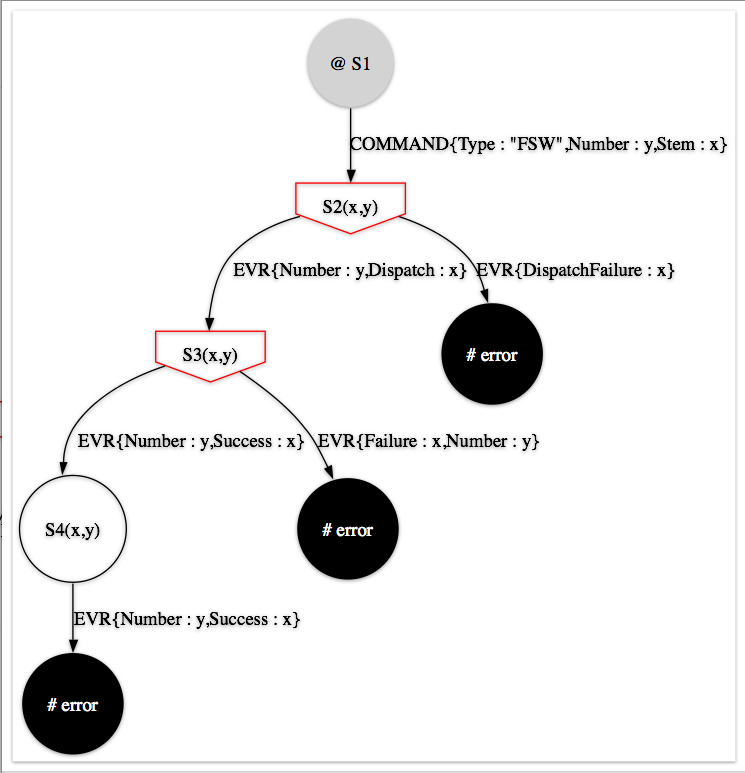
\includegraphics[width=0.8\textwidth]{graphics/A_P3}
\caption{GraphViz view of Automaton A\_P3}
\label{fig:vizA_P3}
\end{center}
\end{figure}

Figure \ref{fig:vizA_P4} illustrates the diagram for automaton {\tt A\_P4}. It illustrates a transition having several
new target states, namely the transition from state {\tt Watch} to the four different states: {\tt wD} (wait for a Dispatch), 
{\tt wS} (wait for a Success), {\tt noDF} (no Dispatch Failure) and {\tt noF} (no Failure). The branching is indicated
with a upwards pointing blue-edged triangle, symbolizing and AND-symbol: `$\wedge$': all the four states must lead to satisfaction.

\begin{figure}
\begin{center}
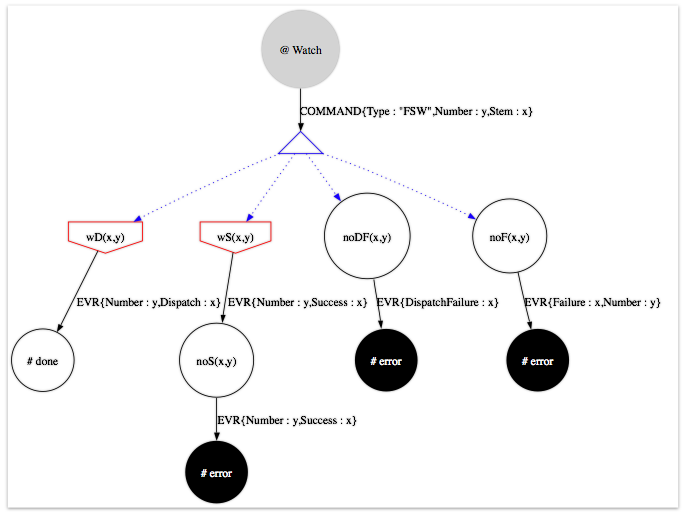
\includegraphics[width=1.0\textwidth]{graphics/A_P4}
\caption{GraphViz view of Automaton A\_P4}
\label{fig:vizA_P4}
\end{center}
\end{figure}


\chapter{The Observer API and its Use}

\section{The Observer API}

The \logscope{} API for monitoring is very simple and consists of three classes: {\tt Observer}, {\tt Results} and {\tt Error} as indicated below (parameter and result types are indicated after colons, where `{\tt +}' means `{\em or}' and `{\tt seq[X]}' means `{\em sequence of X}' - this is not correct \python{}, which is untyped, but helps illustrate the API):

\begin{code}{The \logscope{} Observer API}

def setResultDir(dir : string)
	
class Observer:
  def __init__(self,monitorThis : string+list[string])
  def monitor(self,log : list[dict]) : list[Results]
  def getResults(self) : list[Results]
    
class Results:    
  def getSpecName(self) : string
  def getErrors(self) : list[Error]

class Error:
  def getLocation(self)
  def getMessage(self)
\end{code}	    

\noindent The  {\tt Observer} class gets instantiated with one or more specification file names, and thereafter provides a method {\tt monitor} which can be applied to an event log, which it will check against the specifications. The {\tt monitor} method returns a list of {\tt Results}
objects, one for each specification unit monitored. Each such {\tt Results} object gives access to the name of the specification unit as well as a (possibly empty) list of {\tt Error}s.
The list of {\tt Results} objects returned by the {\tt monitor} method can also be accessed
after monitoring by calling the {\tt getResults} method.

\vspace{0.5cm}

\noindent The {\tt monitorThis} argument to the {\tt Observer} constructor must be either:

\begin{itemize}
  \item a string : denoting an absolute name of a file containing a specification in \logscopeSL.
  \item a sequence of strings (in square brackets -- {\tt [...]}): denoting absolute names of files containing specifications. These specifications will then be joined into one. 
\end{itemize}

\noindent Note that the results of a monitoring run are stored in the text file {\tt RESULTS}
in the result directory set by the {\tt setResultDir(dir : string)} function. This access to the results is sufficient in many cases. However, the API does provide the possibility of accessing the results as data objects (the {\tt getResults} method for example), which may
be useful in regression testing where lots of scripts are run automatically.


\section{An Example Script}

Below is an example of using this API.

%%%%%%%%%%%%%%%%%%
%%%%%%%%%%%%%%%%%%

\label{script}

\begin{code}{An example Python script}

import lsm.lsm as lsm

# create an event log, in this case hand-made, but can also be 
# extracted with log file extractor:

log = [
    \{"OBJ_TYPE" : "COMMAND", 
         "Type" : "FSW", "Stem" : "PICT", "Number" : 231\},
    \{"OBJ_TYPE" : "EVR", "Dispatch" : "PICT", "Number" : 231\},
    \{"OBJ_TYPE" : "CHANNEL", "DataNumber" : 5\},
    \{"OBJ_TYPE" : "EVR", "Success" : "PICT", "Number" : 231\},
    \{"OBJ_TYPE" : "PRODUCT", "ImageSize" : 1200\}
  ]

# specify absolute path of where results should be stored 
# (.dot files and RESULT file):
           
lsm.setResultDir("$EXAMPLES/results")   

# instantiate the Observer class providing a total path name of 
# specification file:

observer = lsm.Observer("$EXAMPLES/manual-examples")

# call the observer's monitor function on the log:

observer.monitor(log)
\end{code}


\section{The Output Generated by LogScope}

This chapter explains the output generated by \logscope{} and how to access it.
The results of monitoring a log is by default printed to standard output. In addition,
the results are written to a file named {\tt RESULTS}, stored in the directory indicated by
the directory indicated as parameter to the {\tt setResultDir} function.

\subsection{No Errors Detected}

Our original log file on page \pageref{logfile} (same as in the script above) satisfies all the properties {\tt P1},...,{\tt P5} and {\tt A\_P1}, {\tt A\_P3} and {\tt A\_P4}. Here we shall focus on properties {\tt P1} and {\tt P2} (by inserting the keyword {\tt ignore} in front of all the other properties). When checking the log file against these two properties the following output is generated.

\begin{verbatim}
=================================
   parsed specification units:
=================================

pattern P1 :
  COMMAND{Type : "FSW", Stem : x, Number : y} =>
    EVR{Success : x, Number : y}

pattern P2 :
  COMMAND{Type : "FSW", Stem : x, Number : y} =>
    !EVR{Failure : x, Number : y}

=====================================
   translated specification units:
=====================================

automaton P1 {
  always S1 {
    COMMAND{Type : "FSW",Number : y,Stem : x} => S2(x,y)
  }

  state S2(x,y) {
    EVR{Number : y,Success : x} => S3(x,y)
  }

  state S3(x,y) {}

  initial S1
  hot S2
}

automaton P2 {
  always S1 {
    COMMAND{Type : "FSW",Number : y,Stem : x} => S2(x,y)
  }

  state S2(x,y) {
    EVR{Failure : x,Number : y} => error
  }

  initial S1
}

=====================================
   monitoring new log of length 5:
=====================================


============================
       RESULTS FOR P1: 
============================

No errors detected!

Statistics {
  COMMAND :
      {'Type': 'FSW', 'Number': 231, 'Stem': 'PICT'} -> 1
  EVR :
      {'Number': 231, 'Success': 'PICT'} -> 1
}

============================
       RESULTS FOR P2: 
============================

No errors detected!

Statistics {
  COMMAND :
      {'Type': 'FSW', 'Number': 231, 'Stem': 'PICT'} -> 1
}

========================
   Summary of Errors:
========================

P1  :  0  
P2  :  0  

specification was satisfied

5 events processed in 0 minutes and 0.00110 seconds (4545 events/sec)

Results are now being written to the file:
/Users/khavelun/Desktop/MSLRESULT/RESULTS

End of session!
\end{verbatim} 

\noindent That is, the output consists of the following elements:

\begin{itemize}
  \item parsed specification units
  \item automata for all specification units (hand-written as well as generated from patterns)
  \item information during monitoring on the progress, in this case nothing is printed since there are so few events.
  Normally is printed for every 100 event: number of events processed so far / total number of events, and the percentage
  this corresponds to.
  \item the result of the verification for each specification unit
  \item a summary of errors for all specification units and other statistics
\end{itemize}

\noindent The result in this case is that no errors were detected for any of the two patterns. For each specification unit is indicated statistics information indicating for each kind of
event how many events matched conditions in the specification unit for each
set of arguments relevant to the specification unit.

In the result directory is in addition to the {\tt RESULT} file also stored two GrapViz dot files with the names {\tt P1.dot} and {\tt P2.dot}. These can be visualized by 
GraphViz (see instructions \cite{graphviz} for your system), as can be seen in
Figure \ref{fig:viz_P1_P2}, using Mac's GraphViz package.

\begin{figure}
\begin{center}
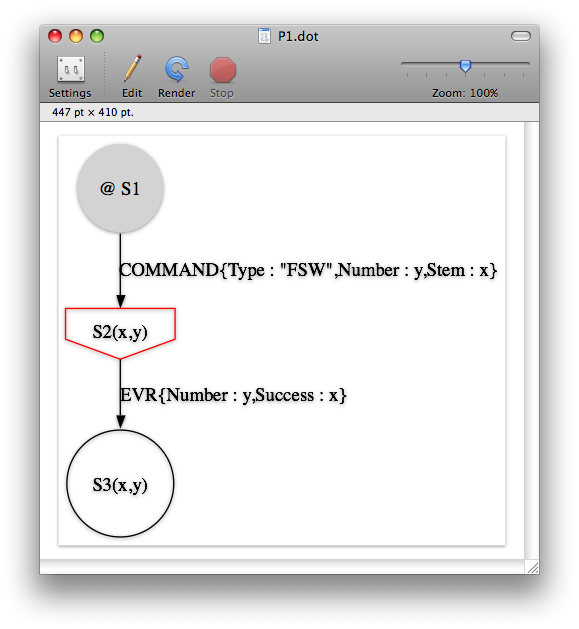
\includegraphics[width=0.6\textwidth]{graphics/P1dot}
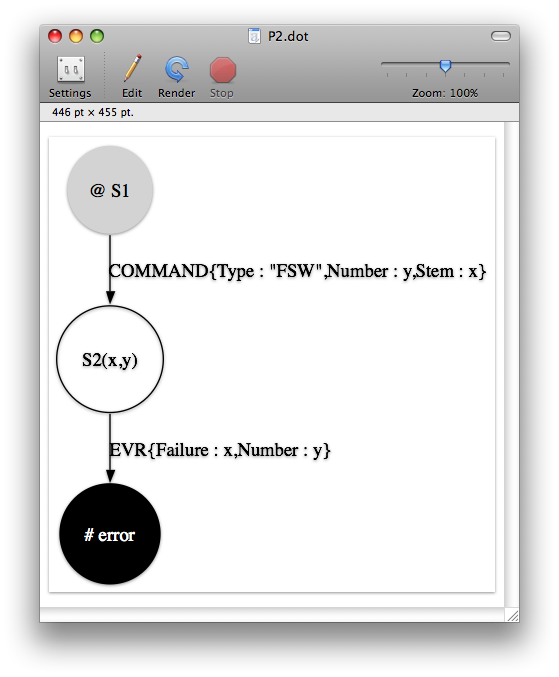
\includegraphics[width=0.6\textwidth]{graphics/P2dot}
\caption{GraphViz view of {\tt P1.dot} and {\tt P2.dot}}
\label{fig:viz_P1_P2}
\end{center}
\end{figure}

\subsection{Errors Detected}

Consider now that we modify the log file in the script on page \pageref{script} 
by changing event number 4 to become a {\em Failure} event instead
of a {Success} event. Note, this is in this example done by  having 
a {\tt Failure} field map to the command name, instead of having
a {\tt Success} field map to the command name. 

\begin{code}{Log with event number 4 indicating failure}

  log = 
   [
    \{"OBJ_TYPE" : "COMMAND",  "Type" : "FSW", 
        "Stem" : "PICT", "Number" : 231\},
    \{"OBJ_TYPE" : "EVR",  "Dispatch" : "PICT", "Number" : 231\},
    \{"OBJ_TYPE" : "CHANNEL",  "DataNumber" : 5\},
->  \{"OBJ_TYPE" : "EVR",  "Failure" : "PICT", "Number" : 231\},
    \{"OBJ_TYPE" : "PRODUCT", "ImageSize" : 1200\}
   ]
\end{code}

\noindent The output of running \logscope{} on this log file and properties {\tt P1} and
{\tt P2} as before is as follows (omitting the listing of the patterns and automata
as these are the same):

\newpage

\begin{verbatim}
=====================================
   monitoring new log of length 5:
=====================================

*** P2 violated: by event 4 in state:

  state S2(x,y) {
    EVR{Failure : x,Number : y} => error
  }
  with bindings: {'y': 231, 'x': 'PICT'}

by transition 1 : EVR{'Failure': 'PICT', 'Number': 231} => error

violating event:

EVR 4 {
  Failure := "PICT" - str
  OBJ_TYPE := "EVR" - str
  Number := 231 - int
}

--- error trace: ---

COMMAND 1 {
  OBJ_TYPE := "COMMAND" - str
  Type := "FSW" - str
  Number := 231 - int
  Stem := "PICT" - str
}

EVR 4 {
  Failure := "PICT" - str
  OBJ_TYPE := "EVR" - str
  Number := 231 - int
}

============================
       RESULTS FOR P1: 
============================

Errors: 1

*** violated: in hot end state:

  state S2(x,y) {
    EVR{Number : y,Success : x} => S3(x,y)
  }
  with bindings: {'y': 231, 'x': 'PICT'}

--- error trace: ---

COMMAND 1 {
  OBJ_TYPE := "COMMAND" - str
  Type := "FSW" - str
  Number := 231 - int
  Stem := "PICT" - str
}

Statistics {
  COMMAND :
      {'Type': 'FSW', 'Number': 231, 'Stem': 'PICT'} -> 1
}

============================
       RESULTS FOR P2: 
============================

Errors: 1

*** violated: by event 4 in state:

  state S2(x,y) {
    EVR{Failure : x,Number : y} => error
  }
  with bindings: {'y': 231, 'x': 'PICT'}

by transition 1 : EVR{'Failure': 'PICT', 'Number': 231} => error

violating event:

EVR 4 {
  Failure := "PICT" - str
  OBJ_TYPE := "EVR" - str
  Number := 231 - int
}

--- error trace: ---

COMMAND 1 {
  OBJ_TYPE := "COMMAND" - str
  Type := "FSW" - str
  Number := 231 - int
  Stem := "PICT" - str
}

EVR 4 {
  Failure := "PICT" - str
  OBJ_TYPE := "EVR" - str
  Number := 231 - int
}

Statistics {
  COMMAND :
      {'Type': 'FSW', 'Number': 231, 'Stem': 'PICT'} -> 1
  EVR :
      {'Failure': 'PICT', 'Number': 231} -> 1
}

========================
   Summary of Errors:
========================

P1  :  1 error 
P2  :  1 error 

specification was violated 2 times

5 events processed in 0 minutes and 0.00121 seconds (4128 events/sec)

Results are now being written to the file:
/Users/khavelun/Desktop/MSLRESULT/RESULTS

End of session!
\end{verbatim}

\noindent We can now see that after event number 4 a violation of P2 is detected:
the automaton for this property is in state {\tt S2} -- with parameters x="PICT" and
y=231, when the listed error transition fires: a failure of the {\tt PICT} command.
The {\em violating failure event} is listed, and then an {\em error trace} showing
the sequence of event from the start of monitoring that drove the monitor into an error state, leaving out events that did not influence the monitor (in this case events 2 and 3).

At the end of monitoring the results for each property are listed. This includes two kind
of errors:

\begin{itemize}
  \item {\em safety properties}: error transitions caused by execution of transitions with 
  {\tt error} on the right hand side. This means that events that should not happen,   
  happened.
  \item {\em liveness properties}: staying in a {\em hot} state at the end of the log. This means that some events that should happen, did not happen.
\end{itemize}

For property {\tt P2} the safety property violation that was reported above is repeated,
including violating event and error trace. For property {\tt P1} a liveness property violation
is reported. The automaton ends in the hot state {\tt S2} (see automaton generated from
the pattern) with x bound to {\tt "PICT"} and y bound to 231. The error trace illustrates the events that brought the automaton to this state.

\section{Dynamic Type Errors}

Specifications entered by the user are type checked statically before being run on a log file. This
catches inconsistencies within the specification. We refer to
such type errors as static type errors. There is, however, also a potential for inconsistencies between the specification and the log file, inconsistencies that cannot be detected before the log file is available. We
refer to such type errors as dynamic type errors. Consider the general form of conditions in specifications:

\[
Kind\{field_1 : range_1,\ldots,field_n : range_n\} 
\]
where {\em Kind} is one of:
{\tt COMMAND}, {\tt EVR}, {\tt CHANNEL}, {\tt CHANGE}, {\tt PRODUCT}.
Two forms of dynamic type errors are considered:

\begin{enumerate}
  \item field errors : mention of field not present in the log file, for example caused by misspellings.
  \item range errors : type errors in ranges. These include:
  \begin{enumerate}
     \item basic type inconsistencies: specification range is an integer, but a non-integer occurs in log. 
              Similar for strings.
     \item interval inconsistencies: specification range is an interval 
             (for example: \verb+PRODUCT{ImageSize : [1000,2000]}+), but a non-integer occurs in log.
	\item indexing errors: specification range is an indexing 
	         (for example:\\ \verb+CHANNEL{DataNumber : {0 : 1, 1 :0, 2 : 1}}+ ). 
	         Here there are two sub-forms:
	         \begin{enumerate}
	           \item the log file value indexed into is an integer: in this case the sub-ranges must be $0$s and
	                   $1$s, as in the example above.
	           \item the log file value indexed into is a string: in this case the sub-ranges must be character
	                   values, that is: strings of length 1.
	         \end{enumerate}
  \end{enumerate}
\end{enumerate}

\noindent
Two forms of error messages are produced by the system to expose dynamic type errors:

\begin{enumerate}
  \item Listing of rules that never fired. This may be caused by type errors in the triggering event of a 
           property. Note though that this may not be caused by errors, just by events that never occur.
  \item Listing of range type errors.
\end{enumerate}

\noindent
The following example illustrates this. Consider the log file on page \pageref{script} of our through-going example. Consider that this is checked against the following two wrongly typed properties 
(errors are explained as comments, referring to the numbered classification above):

\begin{code}{}
pattern P8:  
  COMMAND\{Type : "FSW", Stem: x, number: y\} => 
   # 1: Number misspelled as number
    EVR\{Success: x, Number: y\}  

pattern P9 :
  COMMAND{Type: "FSW", Stem: "PICT"} => 
    \{
      EVR\{Success : \{0 : "FSW"\}, Number : "231"\}, 
       # 2c-ii: Success in log is a string, "FSW" not a char
       # 2a: Number in log is an int, "231" is not
      CHANNEL\{DataNumber : \{0 : "1"\}\}, 
       # 2c-i: DataNumber in log is an int, "1" is not 0 or 1
      PRODUCT\{Stem : [1000,2000]\}  
       # 2b: Stem in log is a string, cannot be in interval  
    \}
\end{code}

\noindent
Although integer versus string errors are reported, \logscope{} does perform auto-conversion from
strings containing numbers to numbers where needed. For example, in property
{\tt P9} above, the {\tt Number} field in the {\tt EVR} event is specified to contain the string
{\tt "231"}, whereas the log contains the number 231. Although this is reported as a dynamic type error,
a conversion is made such the the event does match this particular constraint.

\vspace{0.3cm}

\noindent
Applying \logscope{} to this specification and the log file on page \pageref{script} reports a liveness error
(the {\tt EVR} is not seen) and a safety error (the {\tt PRODUCT} event is not seen), both
caused by our typing errors. In addition, the dynamic typing errors are reported on 
standard output:

\begin{verbatim}
    1 specification(s) never fired.

    Dynamic range type errors: 3.
\end{verbatim}

\noindent
Detailed information about these dynamic type errors is written to the results file as follows:

\begin{verbatim}
==========================
   Dynamic Type Errors:
==========================

The following specifications never fired:
  P8

P9.DataNumber : result of indexing into number must be 0 or 1 
CHANNEL{DataNumber : {0:"1"}}
CHANNEL 3 {
  DataNumber := 5 - int
  OBJ_TYPE := "CHANNEL" - str
}

P9.Number : string or unicode expected - saw int 
EVR{Number : "231",Success : {0:"FSW"}}
EVR 4 {
  OBJ_TYPE := "EVR" - str
  Number := 231 - int
  Success := "PICT" - str
}

P9.Success : result of indexing into string must be a char 
EVR{Number : "231",Success : {0:"FSW"}}
EVR 4 {
  OBJ_TYPE := "EVR" - str
  Number := 231 - int
  Success := "PICT" - str
}
\end{verbatim}

\noindent
It explains that property {\tt P8} never fired (due to the misspelling of {\tt Number} as {\tt number}).
Furthermore, the three dynamic range type errors are listed. For each is explained the name of the property,
the field, the error message, the condition it concerns, and the event that violated the
typing. For example, the first type error (here repeated):

\begin{verbatim}
P9.DataNumber : result of indexing into number must be 0 or 1 
CHANNEL{DataNumber : {0:"1"}}
CHANNEL 3 {
  DataNumber := 5 - int
  OBJ_TYPE := "CHANNEL" - str
}
\end{verbatim}

\noindent
concerns property {\tt P9}, specifically the {\tt DataNumber} field,
and the error message: {\tt result of indexing into number must be 0 or 1}.
Then the conflicting specification condition \verb+CHANNEL{DataNumber : {0:"1"}}+,
and log event: \verb+CHANNEL 3{...}+, are shown, indicating that it is log event number 3.
The problem here is that the string \verb+"1"+ should have been the number \verb+1+ (without quotes).
In this particular case, since \verb+"1"+ contains a number, auto-conversion is applied, and the constraint
matches (which is why there is not reported a missing \verb+CHANNEL+ event).

\vspace{0.3cm}

\noindent
Type checking does slow down monitoring somewhat. It can be turned off by the following
statement at the beginning of the \python{} test script:

\begin{verbatim}
  Options.runtypecheck = False
\end{verbatim}

\chapter{Specification Learning}

Writing specifications can be difficult and time consuming, the key problem being
to identify what properties to check - even just formulated in English prose.
In some cases we may want to learn a specification from  one or more ``{\em well behaved}'' log files, and then later turn this specification into a monitor to check
subsequent log files as part of a regression test suite. \logscope{} provides functionality supporting learning of specifications from logs.

Two forms of learning can be considered: {\em concrete learning} and {\em abstract learning}.
During {\em concrete learning} \logscope{} learns the exact log files it sees up to equivalence on a set of field names that is provided to the learner, either a default set, or field names (for each kind of event) provided
by the user. This results in typically very large learned automata, in principle representing the set of all logs seen during learning, but  projected to the fields of interest. This closely resembles the process one would apply by comparing log files with UNIX's {\tt diff} command after irrelevant event fields have been eliminated for example with UNIX's {\tt grep} command. One will for example be able
to perform some tests on the flight simulator, learning the spec, and then later go into the testbed and carry out the same test, now comparing the new test with the learned spec.
In abstract learning mode one would want for example to learn high level properties about consequences of individual commands, yielding typically small human readable specification units. This abstract learning capability will be provided in a future version of
\logscope{}.

\section{The Learner API}

The concrete Learner API consists of the class {\tt ConcreteLearner}:

\begin{code}{The concrete learner API}

class ConcreteLearner:
  def __init__(self,automatonName : string,
                    fileName : string+None = None)
  def learnlog(self,log : list[dict])
  def dumpSpec(self,filename : string)
\end{code}      

\noindent The constructor takes two arguments, the second of which is optional.
The first argument is the name of the automaton that should be learned. The second
argument indicates the name of a file. If the second file name argument is absent (or {\tt None}), a new automaton will be constructed. If on the other hand the second file name argument is present (a string), the automaton will be read in from that file, and further refined. In the latter case the file must contain an automaton/pattern with the name given as the first argument.

The {\tt learnlog} method takes as argument a log (list of events) and updates the specification accordingly, adding what it sees in the log. This method can be called repeatedly on different logs before the accumulated specification is finally written to a file
with the {\tt dumpSpec} method, taking an absolute file name as argument. This filename
is what subsequently may be passed as the second argument to another call
of the {\tt ConcreteLearner} constructor in order to refine the specification through additional learning.


\section{An Example Script}

The following script illustrates a session using the {\tt ConcreteLeaner} class.

\begin{verbatim}
import lsm.lsm as lsm
          
# create event logs, in this case hand-made for illustration; 
# will typically be extracted with log file extractor:

log1 = [
  {"OBJ_TYPE" : "COMMAND", "Stem" : "PICT"},
  {"OBJ_TYPE" : "EVR", "Dispatch" : "PICT", "EventId" : 2, 
      "Module" : "dispatcher", "Message" : "dispatch done!"},
  {"OBJ_TYPE" : "CHANNEL", "ChannelId" : 3, "DataNumber" : 5},
  {"OBJ_TYPE" : "EVR", "Success" : "PICT", "EventId" : 3,
      "Message" : "command succeeded!"},
  {"OBJ_TYPE" : "PRODUCT", "Name" : "Image", "ImageSize" : 1200}
]

log2 = [
 {"OBJ_TYPE" : "COMMAND", "Stem" : "PICT"},
 {"OBJ_TYPE" : "EVR", "Dispatch" : "PICT", "EventId" : 2, 
     "Module" : "dispatcher", "Message" : "dispatch done!" },
 {"OBJ_TYPE" : "CHANNEL", "ChannelId" : 3, "DataNumber" : 6}, # change data number
 {"OBJ_TYPE" : "EVR", "Success" : "PICT", "EventId" : 3, 
     "Message" : "command succeeded!"},
 {"OBJ_TYPE" : "PRODUCT", "Name" : "Image", "ImageSize" : 1200}
]
                 
log3 = [
  {"OBJ_TYPE" : "COMMAND", "Stem" : "PICT"},
  {"OBJ_TYPE" : "EVR", "Dispatch" : "PICT", "EventId" : 2, 
      "Module" : "dispatcher", "Message" : "dispatch done!"},
  # leave out CHANNEL
  {"OBJ_TYPE" : "EVR", "Success" : "PICT", "EventId" : 3, 
      "Message" : "command succeeded!"},
  {"OBJ_TYPE" : "PRODUCT", "Name" : "Image", "ImageSize" : 1200}
]
                 
log4 = [
  {"OBJ_TYPE" : "COMMAND", "Stem" : "PICT"},
  {"OBJ_TYPE" : "EVR", "Dispatch" : "PICT", "EventId" : 2, 
      "Module" : "dispatcher", "Message" : "dispatch done!"},
  {"OBJ_TYPE" : "CHANNEL", "ChannelId" : 3, "DataNumber" : 5},
  {"OBJ_TYPE" : "EVR", "Failure" : "PICT", "EventId" : 3, 
      "Message" : "***command failed!"},
  {"OBJ_TYPE" : "PRODUCT", "Name" : "Image", "ImageSize" : 1200}
]
                    
# specify absolute path of where results should be stored 
# (.dot files and RESULT file):
          
resultdir = "/Users/khavelun/Desktop/MSLRESULT"
lsm.setResultDir(resultdir)
        
# default fields learned from:
# - for COMMAND : "Stem"
# - for EVR : "EventId","Module","Message","EventNumber"
# - for CHANNEL : "ChannelId","Module","DataNumber"
# - for CHANGE : "ChannelId","Module","DataNumber"
# - for PRODUCT : "Name"

# specify if this should be changed:

lsm.fieldsEVR(["EventId","Module","Message"])
              
# learn a new automaton based on log1 and log2 in the same run:

learner = lsm.ConcreteLearner("LogPattern")
learner.learnlog(log1)
learner.learnlog(log2)
learner.dumpSpec(resultdir + "/LogPattern1.spec")

# refine the spec just stored in LogPattern1.spec by learning from 
# a new log file. store result in LogPattern2.spec.

learner = lsm.ConcreteLearner("LogPattern",resultdir + "/LogPattern1.spec")
learner.learnlog(log3)
learner.dumpSpec(resultdir + "/LogPattern2.spec")

# monitor now a good (log1) and a bad (log4) log file:
        
obs = lsm.Observer(resultdir + "/LogPattern2.spec")
obs.monitor(log1)
obs.monitor(log4)
\end{verbatim}

\section{The Output Generated by \logscopeLearner}

The learned specification is shown below. It describes the 
combined behavior of {\tt log1}, {\tt log2} and {\tt log3}. 
Figure \ref{fig:viz_learned_specs} shows the GraphViz view of the 
dot files of the two learned specifications (the script contains two learning sessions). The top automaton illustrates the result of learning from {\tt log1} and {\tt log2},
while the bottom automaton (equivalent to the one shown in textual format) 
illustrates the result of additionally learning from {\tt log3}. States colored red have been
learned during the most recent learning session. This can also be seen from the
state names, which have the form {\tt L<session number>\_<state number>}, where the
session number increases by 1 for each new learning session.

\newpage

\begin{figure}[htbp]
\begin{center}
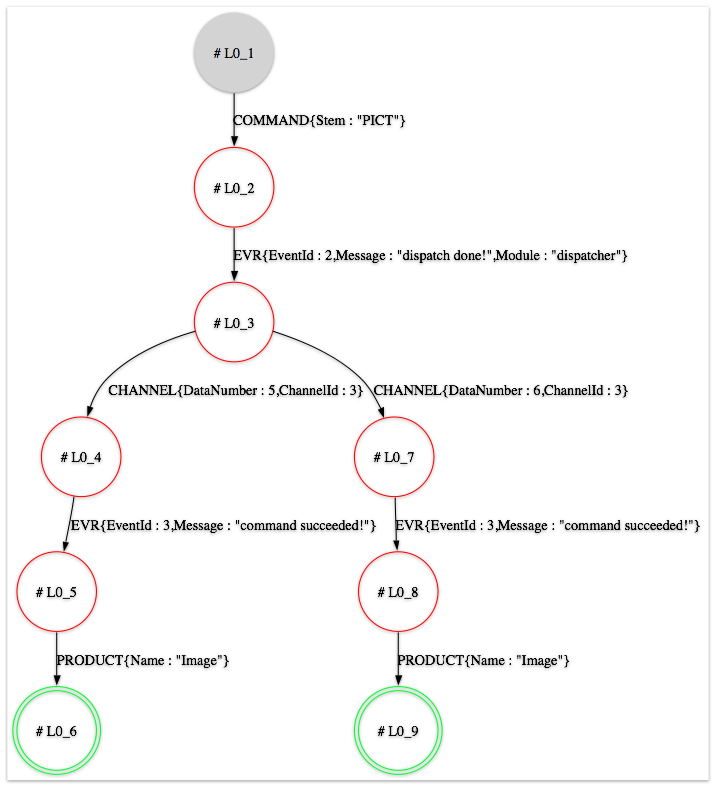
\includegraphics[width=0.7\textwidth]{graphics/LearnedPattern1}
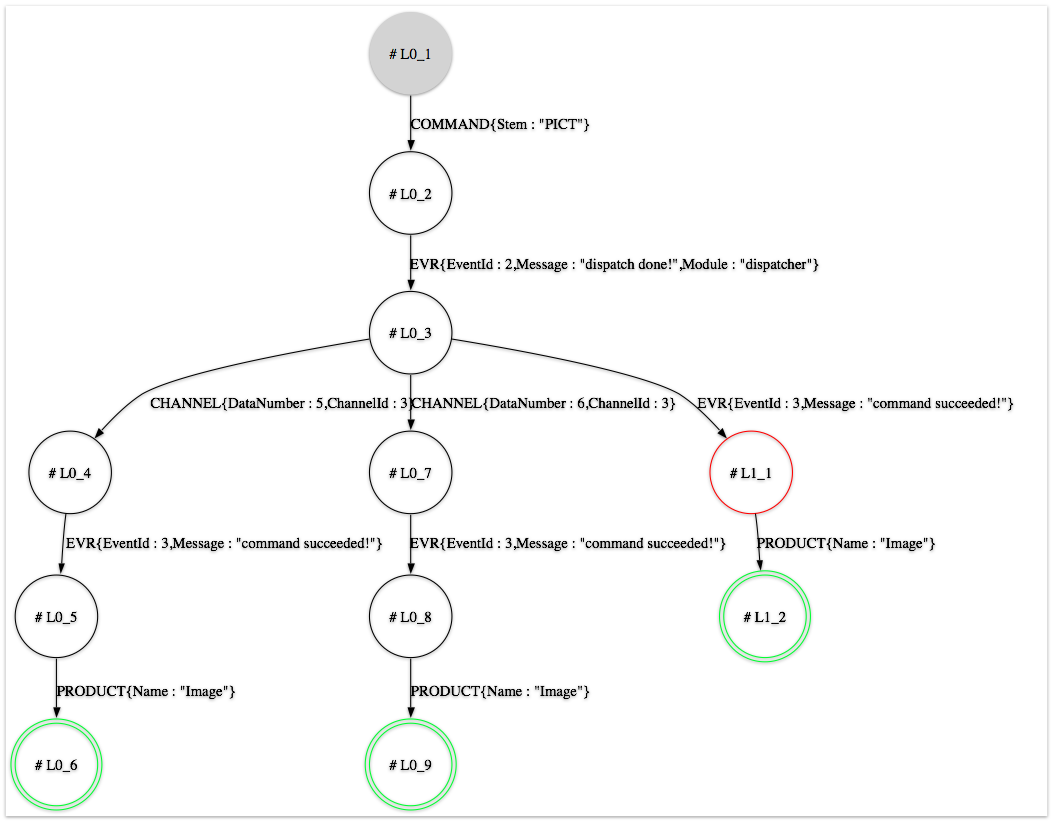
\includegraphics[width=1.0\textwidth]{graphics/LearnedPattern2}
\caption{GraphViz view of {\tt LogPattern1.spec.dot} and {\tt LogPattern2.spec.dot}}
\label{fig:viz_learned_specs}
\end{center}
\end{figure}

\newpage

\begin{code}{}
automaton LogPattern \{
  step L0_1 \{
    COMMAND\{Stem : "PICT"\} => L0_2
  \}

  step L0_2 \{
    EVR\{EventId : 2,Message : "dispatch done!",
          Module : "dispatcher"\} => L0_3
  \}

  step L0_3 \{
    CHANNEL\{DataNumber : 5,ChannelId : 3\} => L0_4
    CHANNEL\{DataNumber : 6,ChannelId : 3\} => L0_7
    EVR\{EventId : 3,Message : "command succeeded!"\} => L1_1
  \}

  step L0_4 \{
    EVR\{EventId : 3,Message : "command succeeded!"\} => L0_5
  \}

  step L0_5 \{
    PRODUCT\{Name : "Image"\} => L0_6
  \}

  step L0_6 \{\}

  step L0_7 \{
    EVR\{EventId : 3,Message : "command succeeded!"\} => L0_8
  \}

  step L0_8 \{
    PRODUCT\{Name : "Image"\} => L0_9
  \}

  step L0_9 \{\}

  step L1_1 \{
    PRODUCT\{Name : "Image"\} => L1_2
  \}

  step L1_2 \{\}

  initial L0_1
  success L0_6,L0_9,L1_2
\}
\end{code}


\appendix

\chapter{\logscopeSL{} Grammar}
\label{app:grammar}

\begin{verbatim}
/* --- lexical elements --- */

NAME = [a-zA-Z_.][a-zA-Z0-9_.]*

NUMBER = [0-9]+

STRING = "..."


/* --- specifications */


specification ::= [pythoncode] monitor+

pythoncode ::= '{:' ... python code ... ':}'

monitor ::= ['ignore'] monitorspec

monitorspec ::= pattern | automaton


/* --- patterns --- */

pattern ::= 
    'pattern' NAME ':' event '=>' consequence ['upto' event]

consequence ::= ['!'] event
              | '[' consequence+, ']'
              | '{' consequence+, '}'

event ::= type '{' constraint*, '}' ['where' predicate] ['do' code]

type ::= 'COMMAND' | 'EVR' | 'CHANNEL' | 'CHANGE' | 'PRODUCT'

constraint ::= NAME ':' range

range ::=  NUMBER 
         | STRING
         | NAME
         | '[' NUMBER ',' NUMBER ']'
         | '{' bitvalue*, '}'

bitvalue ::= value ':' range

value ::= NUMBER | STRING

predicate ::= NAME '(' argument*, ')'
            | pythoncode 
            | predicate 'and' predicate
            | predicate 'or' predicate
            | 'not' predicate
            | '(' predicate ')'

code ::= NAME '(' argument*, ')'
       | pythoncode 

argument ::= NUMBER | STRING | NAME


/* --- automata --- */

automaton ::= 
  'automaton' NAME '{' 
     state* 
     ['initial' action+] 
     ['hot' name+,] 
     ['success' name+,] 
  '}'

state ::= modifier* statekind NAME ['(' name+, ')'] '{' rule* '}'

modifier ::= HOT | INITIAL

statekind ::= 'always' | 'state' | 'step'

rule ::= event '=>' action+,

action ::= NAME ['(' argument*, ')'] | 'done' | 'error'
\end{verbatim}


\chapter{Predefined Predicates}
\label{app:predicates}

\begin{verbatim}
### built-in predicates: ###

def less(x,y):
    return x < y

def equal(x,y):
    return x == y 

def less_equal(x,y):
    return x <= y

def greater(x,y):
    return x > y

def greater_equal(x,y):
    return x >= y

def contains(s,t):
    return s.find(t) != -1

### shorter versions: ###

lt = less
eq = equal
le = less_equal
gt = greater
ge = greater_equal
\end{verbatim}

\bibliographystyle{plain}
\bibliography{biblio}

\end{document}
